\section{Definitions}
\label{Sec:graph_definition}

Graph states can be defined in two ways: through \emph{the stabilizer formalism} or using \emph{quantum circuits}.

\subsection{Stabilizer Formalism Definition}

A stabilizer is an operator under which the stabilised state is invariant, and the state is uniquely specified as the simultaneous $+1$ eigenstate of all $N$ stabilisers,
\begin{equation}
    S_i \ket{\psi} = \ket{\psi} \quad \forall i \in \{1, \ldots, N\} .
\end{equation}

A graph state, described by the graph $G = (V, E)$ has stabilizers of the form
\begin{equation}
    S_i = X_i \otimes_{j \in \mathcal{N}(i)} Z_j ,
\end{equation}
for each node $i$ of the graph, where $\mathcal{N}(i)$ denotes the neighbourhood of the node $i$.

\begin{figure}
    \centering
    

\tikzset{every picture/.style={line width=0.75pt}} %set default line width to 0.75pt        

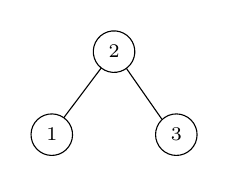
\begin{tikzpicture}[x=0.75pt,y=0.75pt,yscale=-1,xscale=1]
%uncomment if require: \path (0,300); %set diagram left start at 0, and has height of 300

%Shape: Circle [id:dp2524407142420394] 
\draw   (87.86,66.18) .. controls (84.45,70.52) and (78.17,71.28) .. (73.82,67.86) .. controls (69.48,64.45) and (68.72,58.17) .. (72.14,53.82) .. controls (75.55,49.48) and (81.83,48.72) .. (86.18,52.14) .. controls (90.52,55.55) and (91.28,61.83) .. (87.86,66.18) -- cycle ;
%Shape: Circle [id:dp4347791615686073] 
\draw   (41.84,94.21) .. controls (45.04,89.71) and (51.28,88.65) .. (55.79,91.84) .. controls (60.29,95.04) and (61.35,101.28) .. (58.16,105.79) .. controls (54.96,110.29) and (48.72,111.35) .. (44.21,108.16) .. controls (39.71,104.96) and (38.65,98.72) .. (41.84,94.21) -- cycle ;
%Shape: Circle [id:dp6645570183850392] 
\draw   (101.66,105.51) .. controls (98.61,100.91) and (99.88,94.7) .. (104.49,91.66) .. controls (109.09,88.61) and (115.3,89.88) .. (118.34,94.49) .. controls (121.39,99.09) and (120.12,105.3) .. (115.51,108.34) .. controls (110.91,111.39) and (104.7,110.12) .. (101.66,105.51) -- cycle ;
%Straight Lines [id:da7381513422337581] 
\draw    (85.94,68.05) -- (103,92.5) ;
%Straight Lines [id:da16373455646283308] 
\draw    (73.82,67.86) -- (55.79,91.84) ;

% Text Node
\draw (50,100) node  [font=\scriptsize]  {$1$};
% Text Node
\draw (80,60) node  [font=\scriptsize]  {$2$};
% Text Node
\draw (110,100) node  [font=\scriptsize]  {$3$};


\end{tikzpicture}
    \vspace{-1cm}
    \caption{A $3$-qubits linear graph state}
    \label{fig:simple_3_graph}
\end{figure}

As an example, consider the graph in \cref{fig:simple_3_graph}.
The graph state $\ket{G}$ has the stabilizers of the form
\begin{align}
    S_1 &= X_1 \otimes Z_2 , \notag \\
    S_2 &= Z_1 \otimes X_2 \otimes Z_3 , \label{eq:stabilizers} \\
    S_3 &= Z_2 \otimes X_3 , \notag
\end{align}
meaning that
\begin{equation}
    S_1 \ket{G} = 
    S_2 \ket{G} = 
    S_3 \ket{G} = 
    \ket{G} .
\end{equation}

\subsection{Quantum Circuit Definition}

An alternative and equivalent definition is the following.

Given a graph $G = (V, E)$, the graph state $\ket{G}$ is defined by
\begin{equation}
    \ket{G} = \prod_{\substack{\{ a, b \} \in E}} 
    CZ_{a, b} \ket{+}^{\otimes V} ,
\end{equation}
where $CZ_{a, b}$ is the controlled-phase operator between the vertices $a$ and $b$, and 
\begin{equation}
    \ket{+} = H \ket{0} = \frac{1}{\sqrt{2}} (\ket{0} + \ket{1}) .
\end{equation}

For instance, the state in \cref{fig:simple_3_graph} is
\begin{align}
    \ket{G} &=
    \prod_{\substack{\{ a, b \} \in E}} CZ_{a,b} \, H_1 H_2 H_3 \ket{000} =
    CZ_{1, 2} CZ_{2, 3} \ket{+++} \\
    &= \frac{1}{\sqrt{8}} 
    (\ket{000} + \ket{001} + \ket{010} - \ket{011} 
    + \ket{100} + \ket{101} - \ket{110} + \ket{111}) . \notag
\end{align}

It is easy to check that this state is indeed stabilized by the stabilizers $S_1$, $S_2$ and $S_3$ in \cref{eq:stabilizers}.
The equivalence of these definitions is demonstrated in the work \cite{graph_state}.
